\section{CCP Design Principles}
\label{s:design}
%
\begin{figure}[t]
\centering
    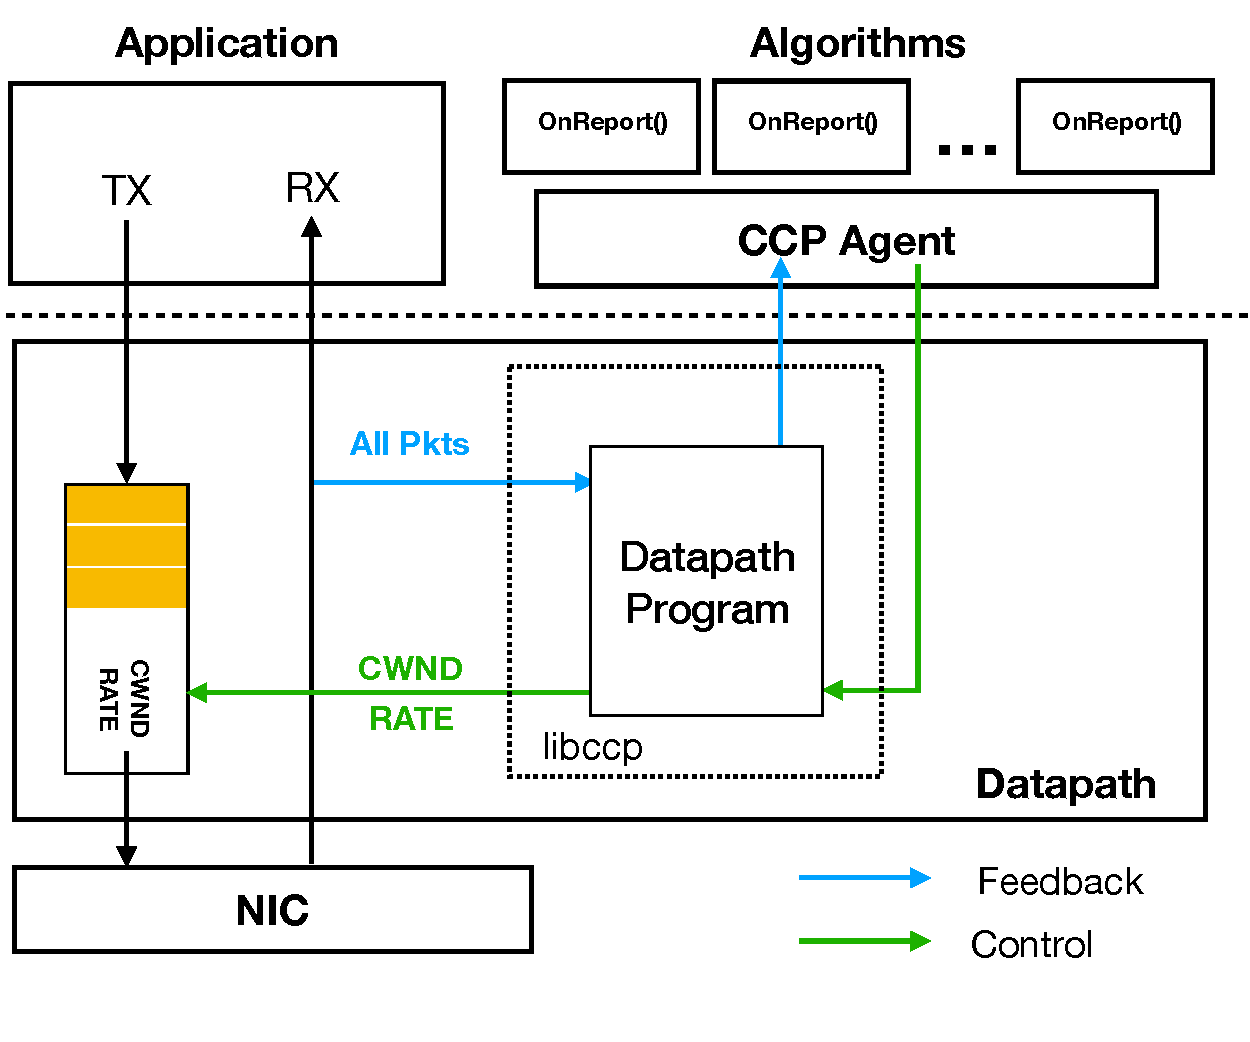
\includegraphics[width=\columnwidth]{img/ccp_design_sigcomm}
    \caption{Congestion control algorithms in CCP are distinct from the application and datapath.
    Users specify control patterns to set the congestion window or rate,
    and fold functions to define how to summarize datapath messages into reports processed in CCP.}\label{fig:design}
\end{figure}
%

To enable rich new congestion control algorithms on datapaths,
CCP must provide a low-barrier programming environment and access
to libraries (\eg for optimization, machine learning, \etc).
%
Further, new algorithms should also achieve high performance running at tens of
Gbit/s per connection with small packet delays in the datapath.

\subsection{Isolating algorithms from the datapath}
\label{s:datapath:isolation}
Should congestion control algorithms run in the same address space as the
datapath? There are conflicting factors to consider:

\Para{Safety.} Supporting experimentation with algorithms and the possibility of
including \userspace library code means that programs implementing congestion
control algorithms should be considered untrusted. If algorithms and the
datapath are in the same address space, bugs in algorithm or library code could
cause datapath crashes or create vulnerabilities leading to privilege
escalations in the kernel datapath.

\Para{Performance.} Congestion control algorithms can access the datapath's
congestion measurements with low delays and high throughput if the two reside in
the same address space.

\Para{Flexibility.} We anticipate future use-cases of the CCP architecture where
a congestion control algorithm may run on a machine different from the sender,
enabling control policies across groups of hosts.

Our design restructures congestion control algorithms into two components in
separate address spaces: an off-datapath {\em CCP agent} and a component that
executes in the datapath itself.
%
The CCP agent provides a flexible execution environment in user space for congestion control algorithms, by receiving congestion signals from the datapath
and invoking the algorithm code on these signals.
%
Algorithm developers have full access to the \userspace programming environment, including tools and libraries.
%
The datapath component is responsible for processing feedback (\eg TCP or QUIC
ACKs, packet delays, \etc) from the network and the receiver, and providing congestion signals to the algorithms.
%
Further, the datapath component provides interfaces for algorithms to set
congestion windows and pacing rates.

An alternative design is to run both the algorithm and the datapath in the same address space, but with fault isolation techniques~\cite{sfi, xfi, bgi, lxfi, nacl, janus, systrace}. 
%
However, this approach comes with significantly increased CPU utilization (\eg 2$\times$ ~\cite{lxfi, sfi, bgi, janus, systrace}, resulting from tracing and run-time checks), a restrictive development environment~\cite{nacl}, or changes to development tools such as the compiler~\cite{xfi, sfi}.
%
These performance and usability impediments, in our view, significantly diminish the benefits of running congestion control algorithms and the datapath in one address space.

\if 0
An alternative design in the case of the kernel datapath, which is to allow
fully functional kernel modules with software fault isolation (\eg
LXFI~\cite{lxfi}) from the rest of the kernel, will likely involve significant
performance impediments.\footnote{Further, an approach such as LXFI also
  requires a careful annotation of kernel functions, and the specification of
  principals and kernel API integrity rules---a challenging task because the
  network stack has a large number of functions with subtle behaviors.}
%
\fi

We believe it is possible to support both designs, but focus on how to achieve high performance
and fidelity when the CCP agent is in a different address space, including the important
case when the datapath is kernel TCP and the CCP agent is in user space.


%% Explicit CCP and datapath separation also enables future use cases where
%% congestion control algorithms may run on a machine different from the sender to
%% centralize congestion control policies across groups of hosts.

%% rephrase the stuff below

\begin{table}[]
    \centering
    \begin{tabular}{c|c|c}
        Implementation & Reporting Interval & Mean Throughput \\
        \hline
        Kernel & - & $43$ Gbit/s \\
        CCP & Per ACK & $29$ Gbit/s \\
        CCP & Per $10$ ms & $41$ Gbit/s \\
    \end{tabular}
    \caption{Single-flow throughput for different reporting intervals between
      the Linux kernel and CCP \userspace, compared to kernel TCP
      throughput. Per-ACK feedback (0 $\mu$s interval) reduces throughput by
      32\% while using a $10$ ms reporting interval
      achieves almost identical throughput to the kernel. Results as the number
      of flows  increases are in
      \S\ref{sec:eval:whyfold}.}\label{tab:perf:interval}
\end{table}

\subsection{Decoupling congestion control from the ACK clock}

Typical congestion control
implementations in the Linux kernel are coupled to the so-called ``ACK-clock,''
\ie algorithm functionality is invoked upon receiving a packet acknowledgment in
the networking stack.

The CCP architecture allows users to express and invoke congestion control logic at a timescale naturally suited to the network (\eg every RTT) and to the algorithmic computation (\eg linear optimization).
%
Algorithms operate over summaries of network observations obtained over multiple ACKs received by the datapath sender.
%
Users program the datapath component in a safe domain-specific language (\S\ref{sec:exercising-control-over-datapath}) to flexibly summarize these observations for the algorithm.

\if 0
While this is also true of a CCP algorithm's fast path, the CCP slow path is
only invoked when the user specifies, whether less frequently than per-ACK or in response to certain urgent conditions.
%
To support this, CCP exposes a \ct{report} instruction for fast path programs to send a
report of the most recent user-defined measurement state in the kernel to the slow path.
\fi

Such decoupling of algorithm logic from the ACK clock provides two benefits.

First, users can develop congestion control algorithms free from the strict
time restrictions rooted in the inter-arrival time of packet acknowledgments---a useful feature, especially at high link rates.
Hence, it becomes possible to implement algorithms that perform complex computations and yet retain high throughput.

Second, providing per-ACK notifications from the datapath to the CCP agent would incur
significant overhead.
%
Table~\ref{tab:perf:interval} shows that for a single saturating \ct{iperf}
connection over a loopback interface, Linux kernel TCP on a server machine
with four 2.8-Ghz cores achieves $45$ Gbit/s running Reno.
%
In comparison, per-ACK reporting from the kernel to the CCP \userspace achieves
only 68\% of the kernel's throughput.
%
By increasing the time between reports sent to the slow path to 10 ms (see the
``per 10 ms'' row), CCP Reno achieves close to the kernel's throughput.

Given that CCP should report measurements only infrequently, a key question is
how best to summarize congestion signals within the fast path, so that CCP
algorithms can achieve high fidelity compared to a baseline that implements the
algorithm completely within the kernel.
Although we are optimistic that a good design can achieve high fidelity because the natural time-scale for end-to-end
congestion control is the RTT between sender and receiver,
achieving it requires a careful design of the datapath component and the information channel between the datapath and the CCP agent.
In \S\ref{sec:eval:fidelity}, we show that using a
larger reporting period does not affect the fidelity of CCP algorithm
implementations relative to native in-kernel implementations.


\subsection{Exercising Control over Datapath Functions}
\label{sec:exercising-control-over-datapath}
\ngs{content below requires some deduplication with section that follows}

% CCP algorithms specify datapath behavior using two mechanisms: {\em fold functions} and {\em control patterns},  whose directives are used by the datapath to summarize congestion signals sent to CCP, and {\em send patterns}, which control packet transmissions on the datapath. 
 
Congestion-control algorithms written in CCP are not tied to the traditional ``ACK clock'', but rather operate on summaries that encapsulate observations over multiple ACKs received by the datapath sender.
CCP algorithms specify datapath behavior using two mechanisms: {\em fold functions} and {\em control patterns}, whose directives are interpreted by the datapath to summarize congestion signals sent to CCP and control packet transmissions on the datapath, respectively. 
 
\paragrapha{Congestion signals and fold functions} All CCP-compatible datapaths should export a well-defined set of congestion signals (Table~\ref{tab:datapath:signals}). There are two kinds of congestion signals: \texttt{Ack} signals, which are computed directly on each ACK (e.g., bytes acked in order, bytes acked out of order, RTT sample, etc.) and \texttt{Flow} signals, which are statistics maintained for the flow (e.g., outgoing and incoming rates). Most of these signals are updated on the arrival of an ACK; the exceptions are: \texttt{was\_timeout} and \texttt{lost\_pkts\_sample} updated on a timeout; and \texttt{bytes\_in\_flight} and \texttt{packets\_in\_flight} updated on packet transmissions.
 
% update others might update on a timeout or at other times. \ma{this is
% vague. what `other times'?}

CCP may read but not write these signals. The only way to gain access to them is via a fold function, which specifies how the datapath should summarize the congestion signals in a single reporting period. 
%For example, a CCP algorithm may ask to receive the sum of the bytes acknowledged in order, the moving average of the RTT samples, and the latest value of the flow's outgoing rate in a reporting period. 
 
%CCP is unaware of how a datapath computes these signals; for example, it does not know which variables the datapath uses to compute the signals. A CCP algorithm, however, specifies how it wants the datapath to summarize each signal over a reporting period using a small language. 
 
%

Fold functions express simple operations over the congestion signal primitives. Table~\ref{tab:datapath:operators} contains the operations each datapath should be able to compute. A CCP algorithm expresses fold functions in a small, restrictive domain-specific language. Each datapath must support this language. For software datapaths, we have developed \texttt{libccp}, a library that provides a reference implementation of fold function computations in this language and other features common to all datapaths (see \S\ref{s:datapath:libccp}). 
 
The fold function defines a structure called \texttt{Summary}. This structure is maintained by the datapath and encapsulates all measurements reported to CCP by the datapath. The CCP algorithm specifies the fields of the \texttt{Summary} structure in the fold function and how to compute each field from congestion signals. The algorithm may define as many fields as it wants in the \texttt{Summary} structure. The datapath writes the values of these fields using the logic supplied by the CCP algorithm.
 
The following fold function shows an example of how to request the number of bytes delivered in order within the reporting period. The sender's datapath runs this function on each received ACK, \texttt{A}:
 
\begin{minted}{lisp}
  (def (Summary.acked 0))
  (:= Summary.acked
    (+ Summary.acked A.bytes_acked))
\end{minted}
 
%The fold function defines a \texttt{Summary} signal, which is the third type of signal maintained by the datapath. 
%Unlike \texttt{Ack} and \texttt{Flow} signals, which are read-only, \texttt{Summary} signals are writeable by the CCP algorithm. 
 
In the example above, the fold function defines a field, \texttt{Summary.acked}, and specifies that on each invocation (typically every received ACK), it should be incremented by the number of in-order bytes observed since the last invocation. After delivering the summary, the datapath resets each reported \texttt{Summary} field to the specified initial value.

Datapath fold functions are written in a restrictive domain-specific language (\Sec{sec:ccp})
that is free from broad classes of vulnerabilities. While \texttt{libccp}, our fast path library (\Sec{s:datapath:libccp}), enforces runtime safety of fast-path algorithm logic,
algorithm implementations are nevertheless free to set arbitrary rates or congestion windows.
As any application can open UDP sockets and congest the network, we do not restrict this behavior.
Meanwhile, CCP \userspace programs have full access to the \userspace programming environment,
tools, and libraries.

%We specify the complete list of available signals and built-in operations on them in \S\ref{s:datapath:fold}.
 
\paragrapha{Control patterns} CCP algorithms can specify the congestion window or pacing rate using simple functions supported by the datapath. These can be set to either absolute values or relative to current values. The algorithms can also specify timing patterns according to which summary reports from fold functions and window/rate settings are executed by the datapath. 
The ability to specify timing patterns is useful for two reasons. First, algorithms may wish to specify patterns of sending; BBR~\cite{bbr}, for example, sends pulses of different magnitudes for specific time durations. Second, algorithms may wish to specify the precise intervals over which congestion signals should be gathered and reported (e.g., once every half-RTT).
 
\begin{minted}{rust}
SetCwndAbs(...) => WaitRtts(0.5) => Report()
\end{minted}
 
Control patterns use \texttt{=>} to specify that the directive on the right should happen after the one on the left. This example pattern uses the \texttt{WaitRtts()} directive to specify that the datapath should set the congestion window to the specified value, wait for a half-RTT, and then report a summary to CCP. After this report, the pattern will reset Summary state and loop back to \texttt{SetCwndAbs()}.
 
%We study this behavior with several experiments in \S\ref{s:eval:fidelity}.
 
Figure~\ref{fig:design} shows the architecture of a CCP-enabled sender, highlighting how the components we have discussed in this section fit together. 



\subsection{Alternative Designs}
\label{sec:design:alternatives}

\an{eBPF is limited and pluggable tcp is strictly less general than us.}

\an{address congestion manager here}


